\chapter{Resultados}
Nesse capítulo os resultados das diferentes soluções propostas no trabalho são apresentados. Primeiramente introduzem-se as medidas de avaliação que serão utilizadas. Em seguida compara-se as etapas de classificação do método tradicional e híbrido, cujo processo de seleção de candidatos é idêntico, portanto a diferença em desempenho se dá apenas no estágio de classificação. Por fim avalia-se o desempenho do sistema completo das diferentes soluções apresentadas.

\section{Medidas de avaliação}
Para avaliar o desempenho das diferentes soluções apresentadas nesse trabalho se faz necessário a utilização de medidas que permitam comparar os resultados objetivamente e indicar facilmente os aspectos positivos e negativos relevantes de cada método. Nesse trabalho tratamos de classificação binária, em que amostras são positivas (representando cabeças e também indicadas por 1) ou negativas (representando não-cabeças e também indicadas por 0). 

Em geral, num problema de classificação o indicador mais comum é a acurácia (\textit{accuracy}), definida \cite{evaluationMetrics} como a razão das classificações corretas pelo total de classificações. É fundamental notar, entretanto, que essa medida sozinha não é suficiente para avaliar um classificador, especialmente se o dataset for desbalanceado. Por exemplo, ao considerar um dataset com duas amostras negativas entre 20 e utilizar um classificador trivial que classifica qualquer amostra como sendo positiva, obtem-se uma acurácia de 90\%, demonstrando o problema dessa métrica.

Uma maneira compacta de representar o desempenho de um classificador é a \textbf{matriz de confusão} \cite{evaluationMetrics}, apresentada na tabela \ref{tab:matriz-confusão}. Para uma classificação binária é uma matriz 2x2 em que a primeira linha indica as amostras negativas e a segunda as amostras positivas. De forma semelhante, a primeira coluna indica amostras que foram classificadas como negativas e a segunda que foram classificadas como positivas. Combinando-se essas linhas e colunas, obtém-se o número de verdadeiros negativos TN, falsos positivos FP, falsos negativos FN e verdadeiros positivos TP, respectivamente. Essa estrutura supera os problemas da acurácia pois fornece a distribuição de acertos e erros de classificação. Adota-se a descrição dos valores em percentuais relativos ao conjunto de análise.

\begin{table}[h]
\centering
\caption{Matriz de confusão}
\label{tab:matriz-confusão}
\begin{tabular}{ll|l|l|}
\cline{3-4}
                                            &   & \multicolumn{2}{l|}{Classificado} \\ \cline{3-4} 
                                            &   & 0               & 1               \\ \hline
\multicolumn{1}{|l|}{\multirow{2}{*}{Real}} & 0 & \text{TN}              & \text{FP}              \\ \cline{2-4} 
\multicolumn{1}{|l|}{}                      & 1 & \text{FN}              & \text{TP}              \\ \hline
\end{tabular}
\end{table}

Outro aspecto a destacar na avaliação de classificadores é que não basta avaliar os indicadores apresentados apenas no conjunto de treinamento. Embora essas medidas forneçam um limite máximo para o desempenho do classificador e permitam detectar \textit{underfitting}, quando o modelo não tem capacidade de modelar o conjunto de treinamento, não se pode avaliar o desempenho do classificador em um caso geral. Por outro lado, se o modelo for demasiadamente complexo ele pode ter se tornado muito específico para algumas características do conjunto de treinamento, situação conhecida como \textit{overfitting}. Assim, para medir o desempenho do classificador em uma situação real utiliza-se de outro conjunto de dados supervisionados chamado de conjunto de teste -- \textit{test set}, independente do conjunto de treinamento. Afirma-se que o modelo generaliza bem se o desempenho no conjunto de treinamento se equiparar ao de teste.

Graficamente pode-se avaliar classificadores através do gráfico ROC -- \textit{Receiver Operating Characteristic} \cite{evaluationMetrics}, que relaciona a taxa de verdadeiros positivos
\begin{equation}
\text{TVP} = \frac{\text{TP}}{\text{FN}+\text{TP}}
\end{equation}
com a taxa de falsos positivos 
\begin{equation}
\text{TFP} = \frac{\text{FP}}{\text{TN}+\text{FP}}.
\end{equation} 
Dessa forma, o classificador ideal indicaria uma TVP unitária com TFP nula, o que caracteriza o ponto $(0,1)$.

A princípio cada classificador avaliado em um conjunto de dados corresponde a um ponto no espaço ROC. Entretanto existem classificadores cuja saída é a probabilidade da amostra ser positiva. Nesses casos é possível escolher um limiar de probabilidade $T$ acima do qual se considera uma amostra como positiva. Cada escolha desse limiar corresponderá a um ponto no espaço ROC e variando esse parâmetro é possível obter uma curva nesse espaço.

Comparar diferentes classificadores não é trivial pois é uma tarefa multiobjetivo que envolve simultaneamente maximizar a TVP e minimizar TFP. Portanto só é possível afirmar que um classificador é melhor do que outro sse sua TVP é maior e sua TFP é menor que a do outro, nesse caso diz-se que o primeiro domina o segundo. Na prática, entretanto, utiliza-se a métrica \textit{Area Under Curve} -- AUC, que mede a área sob a curva ROC, para facilitar essa comparação, especialmente quando a região de operação não é especificada.

Um requerimento específico para a aplicação em questão é que a linha de produção se mantenha em funcionamento o maior tempo possível, para tanto deve-se minimizar a quantidade de falsos positivos FP, que significam cabeças incorretamente identificadas que interrompam a produção sem necessidade. Assim, demanda-se uma TFP menor que 10\%. Quando especificada, a AUC será correspondente à área sob a curva ROC com TFP inferior à esse limite.

\section{Classificadores}
\label{sec:resultados-classificadores}
O classificador SVM originalmente possui saída categórica, porém pode ser adaptado para fornecer uma saída probabilística que indica a probabilidade da amostra ser positiva. Nota-se entretanto que internamente a formulação é ainda categórica. Já os métodos profundos possuem saídas probabilísticas por definição. Essa estrutura da saída como probabilidade é vantajosa pois permite ajustar o compromisso entre falso positivos e falso negativos do classificador, após treinamento, através da escolha do limiar de probabilidade $T$ acima do qual uma amostra é considerada positiva. Escolher um limiar mais alto significa exigir mais segurança do classificador e, portanto, reduzir o número de falsos positivos ao preço de aumentar o número de falsos negativos.

No caso de saídas probabilísticas, para representar a matriz de confusão se faz necessário escolher um limiar $T$. Nesse trabalho escolhem-se dois valores (0.5 e 0.9) para esse parâmetro de maneira a demonstrar sua influência sob a distribuição das amostras na classificação. Nota-se que a estrutura de classificação é a mesma, apenas o limiar é trocado.

Para realizar o treinamento dos classificadores foi gerado um conjunto de dados a partir de gravações realizadas no ambiente indústrial onde o sistema deverá ser instalado. A câmera foi posicionada num ponto próximo de onde deve ocorrer a sua instalação final. Diversos vídeos foram gravados e posteriormente analisados. Utilizando o algoritmo de detecção de candidatos visto em \ref{sec:tradicional-candidatos}, selecionou-se manualmente em cada quadro quais dos candidatos eram verdadeiramente cabeças.

Repetindo esse processo em cada quadro formou-se um conjunto de treinamento, cuja amostra é o recorte do candidato, reduzido de 2459 amostras negativas (não cabeças) e 667 positivas (cabeças). Em seguida estendeu-se esse conjunto reduzido para 9894 amostras negativas e 1222 positivas, formando o conjunto de treinamento completo. Para averiguar o desempenho estendeu-se esse conjunto para 16898 amostras das quais 14966 são negativas. Criou-se, ainda, um conjunto de teste independente de 2738 amostras negativas e 235 amostras positivas.

\subsection{Método tradicional}
Avaliou-se o resultado dos diferentes descritores mencionados em \ref{sec:tradicional-descritores} utilizando um processo de treinamento automático do SVM \cite{scikit-learn}: varreu-se o espaço dos parâmetros $C$ entre $0.0001$ e $0.01$ com passos de $0.001$ e $\sigma$ entre $1$ e $100$ com passos de $5$. Selecionou-se os melhores resultados através da medida conhecida como precisão (\textit{precision}) definida como
\begin{equation}
P = \frac{\text{TP}}{\text{FP}+\text{TP}}
\end{equation}
comumente utilizada e disponível no \textit{toolkit} utilizado.

Primeiramente avaliou-se qual a dimensão do descritor de anéis concêntricos que apresenta melhor resultado. Para tanto treinou-se classificadores SVM de saída probabilística com as descrições em 8, 16 e 18 dimensões sob o conjunto de treinamento reduzido, obtendo as matrizes de confusão das tabelas \ref{cm:aneisR8}, \ref{cm:aneisR16} e \ref{cm:aneisR18}. Obtiveram-se as curvas ROC desses classificadores avaliados no conjunto de teste, vistas na figura \ref{fig:roc-rings}. 

\begin{table}
\cfmat{Anéis concêntricos, 8 dimensões, conjunto de treinamento reduzido}{2364}{65}{185}{482}{cm:aneisR8}
\cfmat{Anéis concêntricos, 16 dimensões, conjunto de treinamento reduzido}{2385}{44}{111}{556}{cm:aneisR16}
\cfmat{Anéis concêntricos, 18 dimensões, conjunto de treinamento reduzido}{2410}{19}{60}{607}{cm:aneisR18}
\end{table}

\begin{figure}
\centering
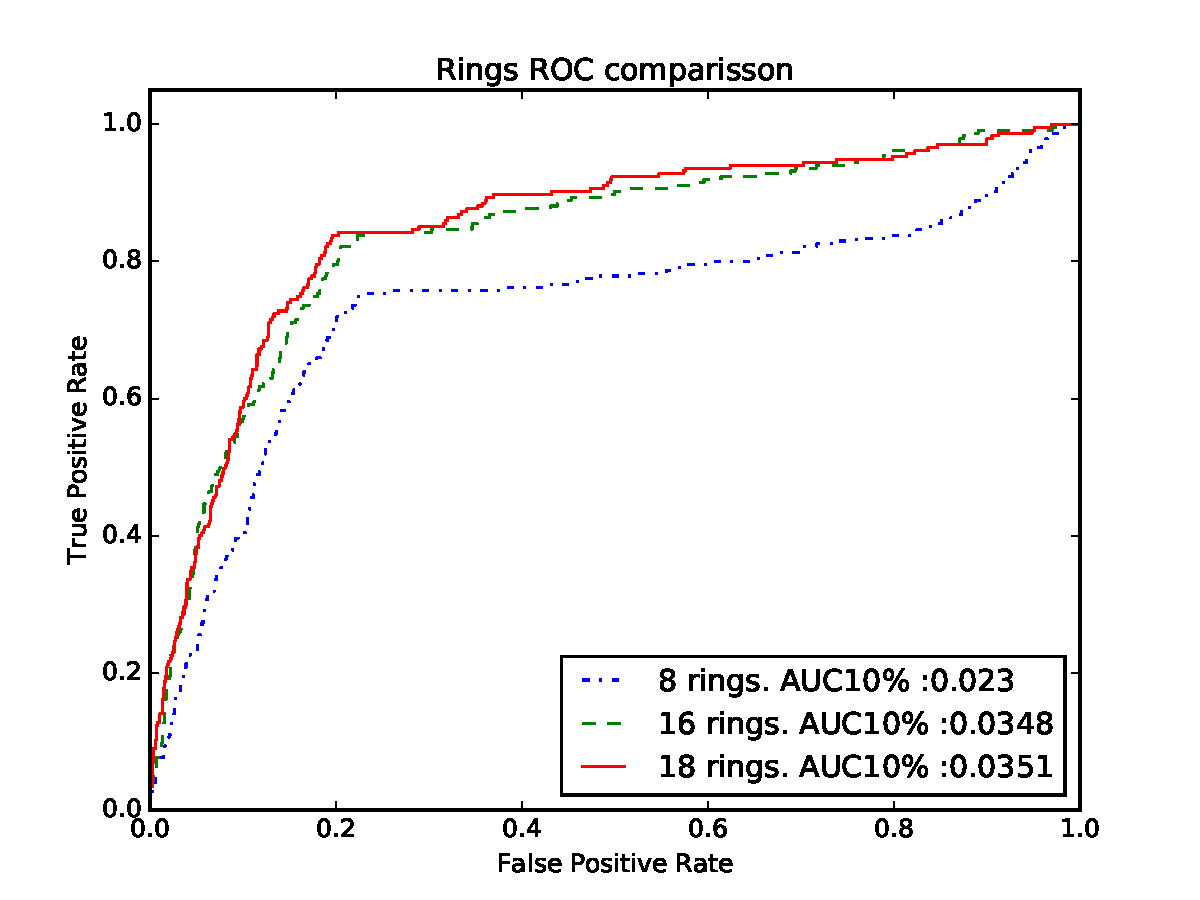
\includegraphics[width=0.8\textwidth]{results/ROC_rings}
\caption{Curvas ROC comparando classificadores SVM sob descritores de anéis com diferentes dimensões.}
\label{fig:roc-rings}
\end{figure}

Tendo visto que o classificador de 18 dimensões domina sob os outros na região de operação com menor TFP, decidiu-se selecionar esse descritor para seguir com a análise. Para tanto utilizou-se o conjunto de treinamento completo para o treinamento e posterior avaliação através do conjunto de teste, como visto nas tabelas \ref{cm:aneis18Tr} e \ref{cm:aneis18Te}.

\begin{table}
\cfmat{Anéis concêntricos com 18 dimensões, conjunto treinamento}{9890}{4}{79}{1143}{cm:aneis18Tr}
\cfmat{Anéis concêntricos com 18 dimensões, conjunto teste}{2564}{174}{158}{77}{cm:aneis18Te}
\end{table}

Outro descritor que também foi avaliado foi o de grades simples com dimensão 7x7, como demonstra as tabelas \ref{cm:gradesTr} e \ref{cm:gradesTe}.

\begin{table}
\cfmat{Grades simples, conjunto treinamento}{9881}{13}{36}{1186}{cm:gradesTr}
\cfmat{Grades simples, conjunto teste}{2445}{293}{181}{54}{cm:gradesTe}
\end{table}

\subsection{Classificador profundo}

\subsubsection{MLP}
Na estrutura MLP foram realizados testes com duas e três camadas intermediárias, com ativação RELU e um único perceptron de saída com ativação sigmoide indicando a probabilidade da amostra ser uma cabeça. Na configuração de duas camadas foram utilizados 512 e 256 perceptrons, respectivamente. Os resultados obtidos para o conjunto de treinamento são apresentados nas tabelas \ref{cm:MLP:Tr:5} e \ref{cm:MLP:Tr:9}. O resultado do conjunto de teste são apresentados nas tabela \ref{cm:MLP:Te:5} e \ref{cm:MLP:Te:9}.

\begin{table}
\cfmat{MLP, conjunto treinamento extendido $T=0.5$}{14533}{433}{104}{1828}{cm:MLP:Tr:5}
\cfmat{MLP, conjunto treinamento extendido $T=0.9$}{14794}{172}{252}{1680}{cm:MLP:Tr:9}

\cfmat{MLP, conjunto teste $T=0.5$}{2489}{249}{10}{225}{cm:MLP:Te:5}
\cfmat{MLP, conjunto teste $T=0.9$}{2635}{103}{25}{210}{cm:MLP:Te:9}
\end{table}

Para três camadas foram utilizados 1024, 512 e 256 perceptrons respectivamente, entretanto os resultados foram semelhantes aos obtidos com duas camadas, portanto o aumento em complexidade não é justificado visto que o desempenho permaneceu o mesmo.

\subsubsection{Redes convolucionais}
Para redes convolucionais utilizou-se uma única camada convolucional RELU com 16 núcleos 3x3 seguida por max-pooling (3x3) e uma camada densamente conectada de 128 percepetrons RELU e finalmente saída única com ativação sigmoide. Essa topologia foi a que teve o melhor desempenho, obtendo 99\% de acurácia no conjunto de treinamento, demonstrados nas tabelas \ref{cm:CNN:Tr:5} e \ref{cm:CNN:Tr:9}. Também teve 96\% de acurácia no conjunto de teste, como observado nas tabelas \ref{cm:CNN:Te:5} e \ref{cm:CNN:Te:9}.

\begin{table}
\cfmat{CNN, $T=0.5$, conjunto treinamento extendido}{14934}{32}{23}{1909}{cm:CNN:Tr:5}
\cfmat{CNN, $T=0.9$, conjunto treinamento extendido}{14950}{16}{113}{1819}{cm:CNN:Tr:9}

\cfmat{CNN, $T=0.5$, conjunto de teste}{2521}{88}{16}{219}{cm:CNN:Te:5}
\cfmat{CNN, $T=0.9$, conjunto de teste}{2691}{47}{34}{201}{cm:CNN:Te:9}
\end{table}


\subsection{Discussão}
Verifica-se as curvas ROC dos classificadores correspondentes avaliados no conjunto de teste na figura \ref{fig:ROC}. Observando a região de interesse (TFP menor que 10\%) fica claro que os métodos profundos, com CNN e MLP, dominam sob os superficiais. Em mais detalhes, MLP domina entre TFP de 0.1\% a 1.3\%, a partir de onde CNN passa a dominar. Para especificar qual o melhor classificador entre os profundos é necessário saber exatamente a região de operação em que se deseja atuar. 

Observa-se que muitos classificadores obtiveram um desempenho elevado no conjunto de treinamento, em especial as redes convolucionais que obtiveram acurácia quase unitária (sob dataset balanceado), demonstrando a alta capacidade do modelo. Nota-se, entretanto, que há grande discrepância entre o desempenho dos classificadores no conjunto de treinamento e de teste nos métodos superficiais, o que caracteriza \textit{overfitting}. Os métodos profundos, em contraste, apresentam uma boa generalização. Isso é explicado porque o modelo em questão foi corretamente especificado através no número de camadas e tamanho de filtros, de forma que sua capacidade se ajuste de forma adequada aos dados.

\begin{figure}
\centering
\begin{subfigure}{.5\textwidth}
  \centering
  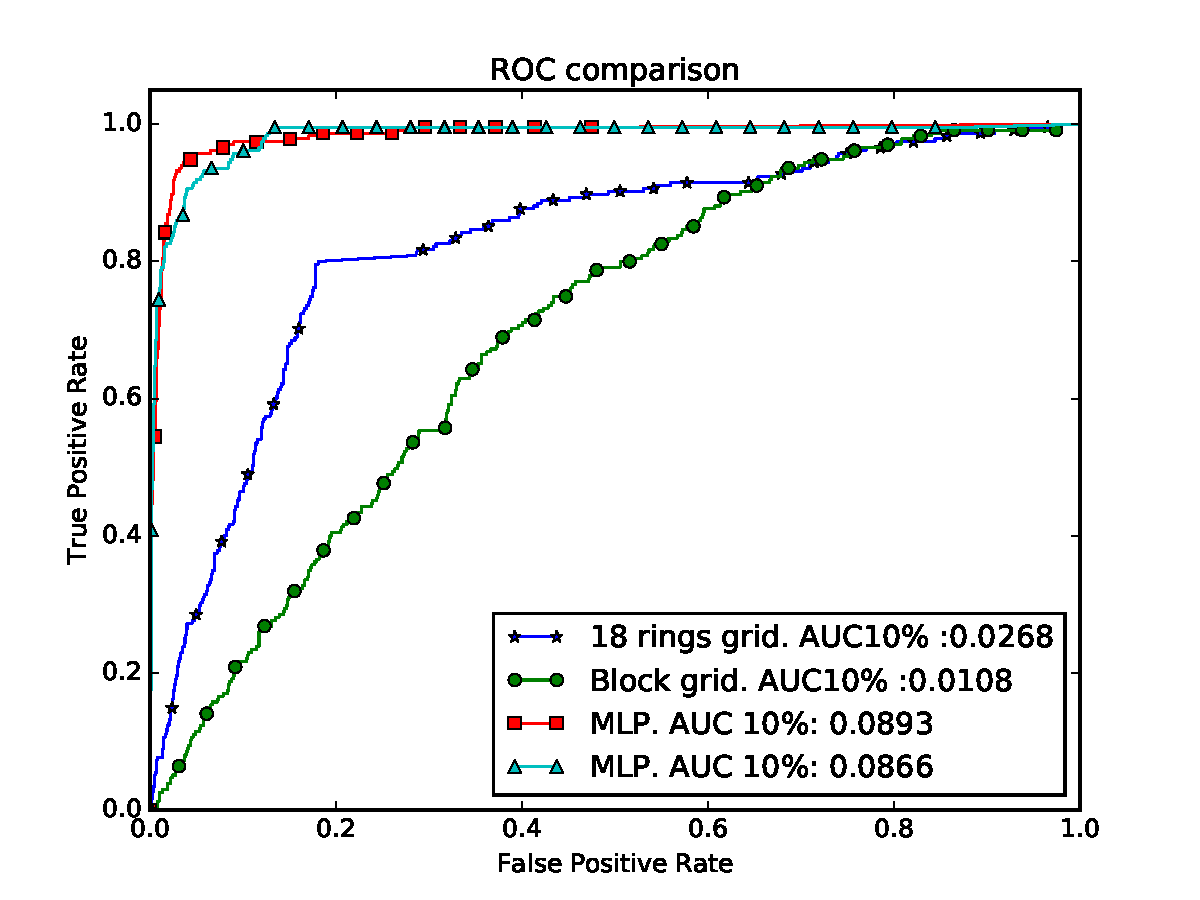
\includegraphics[width=\linewidth]{results/ROC_all}
\end{subfigure}%
\begin{subfigure}{.5\textwidth}
  \centering
  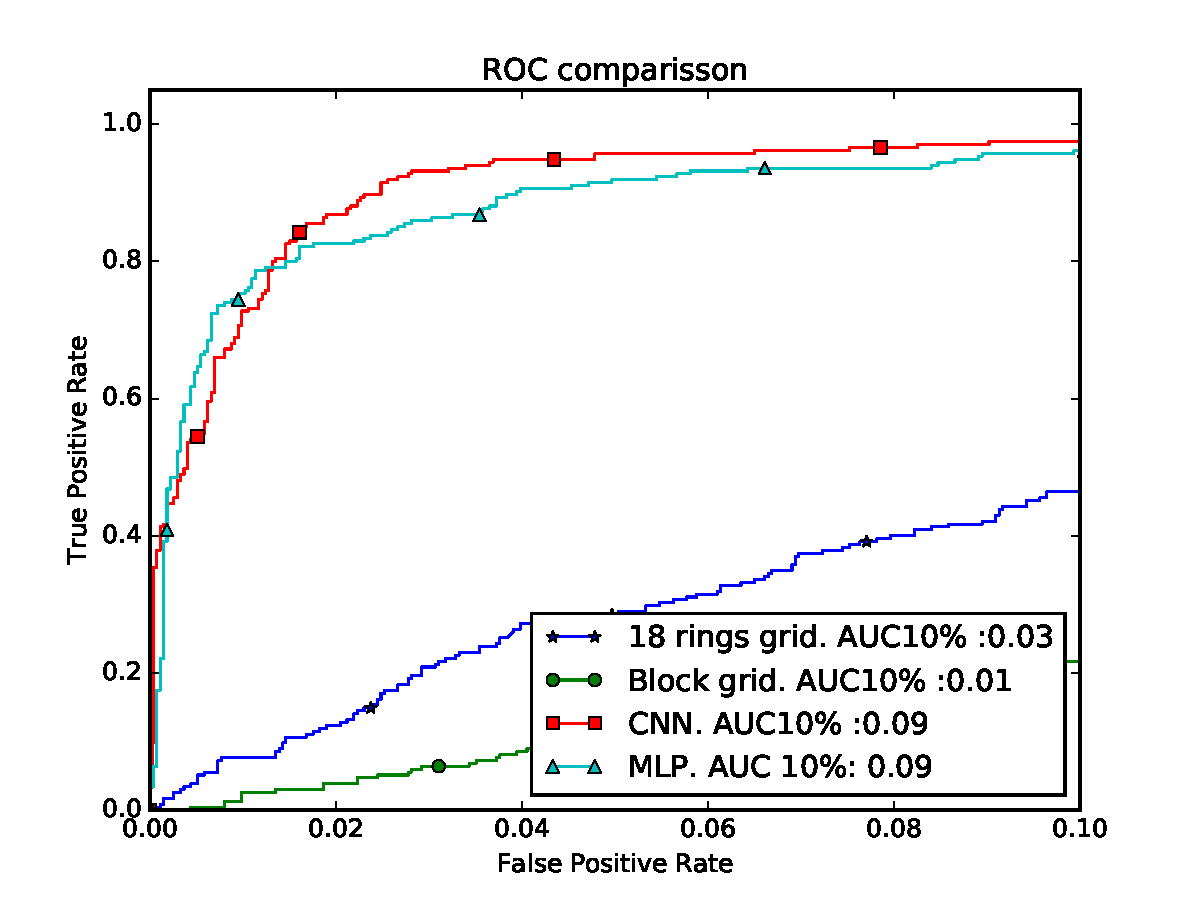
\includegraphics[width=\linewidth]{results/ROC_all_zoom}
\end{subfigure}
\caption{Curvas ROC comparando diferentes classificadores apresentados e zoom na região de interesse}
\label{fig:ROC}
\end{figure}

\section{Sistema completo}
Nessa seção serão comparados os resultados do sistema de extração de candidatos e de classificação como um todo. Tendo em vista os resultados da seção \ref{sec:resultados-classificadores}, a solução baseada na seleção de candidatos vista em \ref{sec:tradicional-candidatos} e classificador CNN apresentada no capítulo \ref{chap:class-profundo} será avaliada em detrimento das demais variações de classificadores. A última solução, cuja detecção e classificação são realizadas utilizando métodos profundos, vista no capítulo X também será avaliada.
